% ADS Project 2 -- Dijkstra with four priority queues
% This report is self-contained and uses data recorded in the repository.

\documentclass[12pt,a4paper]{report}
\usepackage[utf8]{inputenc}
\usepackage[T1]{fontenc}
\usepackage{geometry}
\usepackage{amsmath,amssymb}
\usepackage{graphicx}
\usepackage{booktabs}
\usepackage{float}
\usepackage{caption}
\usepackage{titlesec}
\usepackage{enumitem}
\usepackage{xcolor}
\usepackage{algorithm}
\usepackage{algorithmicx}
\usepackage{algpseudocode}
\usepackage{indentfirst}
\usepackage{multirow}
\usepackage{hyperref}
\usepackage{pgfplots}

\geometry{left=2.5cm,right=2.5cm,top=2.5cm,bottom=2.5cm}
\setlength{\parindent}{2em}
\setlength{\parskip}{1pt}

\titleformat{\chapter}
  {\normalfont\LARGE\bfseries}
  {\chaptername\ \thechapter.\quad}
  {0pt}
  {}
\titlespacing*{\chapter}{0pt}{0pt}{20pt}

\titleformat{\section}
  {\normalfont\large\bfseries}
  {\thesection}
  {1em}
  {}
\titlespacing*{\section}{0pt}{12pt}{6pt}

\titleformat{\subsection}
  {\normalfont\normalsize\bfseries}
  {\thesubsection}
  {1em}
  {}
\titlespacing*{\subsection}{0pt}{10pt}{4pt}

\setlist[itemize]{left=0pt,topsep=4pt,partopsep=0pt,itemsep=2pt}
\setlist[enumerate]{left=0pt,topsep=4pt,partopsep=0pt,itemsep=2pt}

\hypersetup{colorlinks=true,linkcolor=blue,urlcolor=blue,citecolor=blue}
\pgfplotsset{compat=1.18}
\newcommand{\code}[1]{\texttt{\detokenize{#1}}}

\begin{document}

% ------------------------------- title page -------------------------------
\begin{center}
  {\Huge\bfseries Performance Comparison of\\[0.35cm]
   Four Priority Queues for Dijkstra's Algorithm\par}
  \vspace{1.5cm}
  \Large Course: Data Structures and Algorithms\\[0.35cm]
  \Large Project: Shortest Path Algorithm with Heaps\\[0.35cm]
  \Large Implementation: C (C11 / C++17-compatible C style)\\[0.35cm]
  \Large Completion Date: October 25, 2026\\[1.2cm]
  \Large You Longbin \quad 3250106392\\
  \vspace{0.4cm}
  \Large Huang Yirui \quad 3250104426\\
  \vspace{0.4cm}
  \Large Chen Zhikun \quad 3250100883\\
  \vspace{1.5cm}
  \Large Generated with \LaTeX
\end{center}

\newpage
\tableofcontents
\newpage

% ============================== Chapter 1 ================================
\chapter{Introduction}

\section{Description}
The single-source shortest-path problem asks for the minimum path cost from a
source vertex to every other vertex in a weighted graph. When all edge weights
are non-negative, Dijkstra's algorithm solves this problem by repeatedly
selecting the unsettled vertex with the smallest tentative distance and
relaxing its outgoing edges. A min-priority queue supports this selection and
the key updates caused by successful relaxations.

The project asks us to implement Dijkstra's algorithm with multiple heap
structures and determine which implementation performs best on USA road
networks. The evaluation uses three DIMACS graphs, NY, COL, and FLA, with 1,000
distinct source--target queries per graph. The implementation compares four
min-priority queues: binary, ternary, Fibonacci, and binomial heaps. Including
four structures exceeds the assignment's two-structure minimum and includes
the required Fibonacci heap.

The measured task is a point-to-point query rather than a complete single-source
run. Each query terminates as soon as the target is extracted as the current
minimum. This early termination makes the tested workload smaller than a full
traversal and makes the operation mix, query distribution, and queue
implementation important to the result.

\section{Overview of the Implementation}
The program is organized around four shared components.

\begin{enumerate}
  \item \textbf{Graph loading.} The DIMACS road network is parsed into a
        compressed sparse row (CSR) representation. An offset array identifies
        each vertex's outgoing-arc range, while one contiguous edge array stores
        destinations and non-negative weights.
  \item \textbf{Priority queues.} Each heap implements insertion,
        extract-min, decrease-key, and clearing after a query. The two array
        heaps use a vertex-position array; the linked heaps use their tree and
        root-list structures.
  \item \textbf{Dijkstra query runner.} A common search procedure is run with
        each heap. It stops at the target, records high-level operation counts,
        and uses the same deterministic comparison order, $(distance, vertex
        ID)$, for every implementation.
  \item \textbf{Benchmark and output.} A deterministic generator creates the
        query pairs. The program records runtimes, returned distances, and
        Dijkstra-level work in CSV files. A separate count-only build records
        internal heap operations without adding those counter updates to the
        timed build.
\end{enumerate}

Chapter 2 specifies the common search and summarizes the four heaps. Chapter 3
presents the input graphs, evaluation procedure, correctness cross-check,
runtime table, and plot. Chapter 4 focuses on the measured causes of the
performance differences and states the limits of the evidence. The appendix
points to the complete source without duplicating implementation code.

% ============================== Chapter 2 ================================
\chapter{Algorithm Specification}

\section{Graph and Priority-Queue Data Structures}
Let $G=(V,E)$ be a directed graph with non-negative edge weights. The graph is
stored in CSR form: \code{offset[u]} through \code{offset[u+1]-1} index the
outgoing arcs of vertex $u$. The edge array stores the destination and weight
for each arc. This representation requires $O(V+E)$ memory and avoids the
$O(V^2)$ space of an adjacency matrix.

Each queue item is ordered lexicographically by its key and vertex ID. This
gives deterministic tie-breaking when two tentative distances are equal. The
queue API is the same for all four heaps: insert a vertex, extract the
minimum-key item, decrease a queued vertex's key, check whether the queue is
empty, and clear the remaining items after a query.

\begin{table}[H]
  \centering
  \caption{Priority-queue representations and operation costs}
  \label{tab:heap-operations}
  \small
  \begin{tabular}{p{1.7cm}p{4.4cm}p{2.0cm}p{2.3cm}p{2.3cm}}
    \toprule
    Heap & Representation & Insert & Extract-min & Decrease-key \\
    \midrule
    Binary & Array; vertex-position map & $O(\log q)$ & $O(\log q)$ & $O(\log q)$ \\
    Ternary & Array; three-way branching; position map & $O(\log q)$ & $O(\log q)$ & $O(\log q)$ \\
    Fibonacci & Circular root/child lists; consolidation and cuts & $O(1)$ amort. & $O(\log q)$ amort. & $O(1)$ amort. \\
    Binomial & Degree-ordered tree roots & $O(\log q)$ & $O(\log q)$ & $O(\log q)$ \\
    \bottomrule
  \end{tabular}
  \vspace{2pt}

  \footnotesize $q$ denotes the current number of items in the priority queue.
\end{table}

The two array heaps differ only in branching factor. The Fibonacci heap uses
root and child lists with consolidation after extract-min; the binomial heap
uses degree-ordered trees. These structural differences are relevant to the
performance analysis in Chapter 4; implementation-level code is in
\code{src/1.c}.

\section{Dijkstra Query Algorithm}
\noindent\textbf{Input}: Directed graph $G$ with non-negative edge weights,
source $s$, target $t$, and an empty min-priority queue $Q$\\
\textbf{Output}: The shortest-path distance from $s$ to $t$, or $\infty$ if
no path exists

\begin{algorithm}[H]
  \begin{algorithmic}[1]
    \ForAll{$v \in V$}
      \State $dist[v] \gets \infty$
      \State $state[v] \gets \text{UNSEEN}$
    \EndFor
    \State $dist[s] \gets 0$
    \State \Call{Insert}{$Q,s,0$}
    \State $state[s] \gets \text{IN\_QUEUE}$
    \While{$Q$ is not empty}
      \State $(u,d) \gets$ \Call{ExtractMin}{$Q$}
      \State $state[u] \gets \text{SETTLED}$
      \If{$u=t$}
        \State \Return $d$
      \EndIf
      \ForAll{arcs $(u,v,w)$ leaving $u$}
        \If{$state[v] \neq \text{SETTLED}$ and $d+w < dist[v]$}
          \State $dist[v] \gets d+w$
          \If{$state[v] = \text{UNSEEN}$}
            \State \Call{Insert}{$Q,v,dist[v]$}
            \State $state[v] \gets \text{IN\_QUEUE}$
          \Else
            \State \Call{DecreaseKey}{$Q,v,dist[v]$}
          \EndIf
        \EndIf
      \EndFor
    \EndWhile
    \State \Return $\infty$
  \end{algorithmic}
  \caption{Point-to-point Dijkstra query with early termination}
  \label{alg:dijkstra-query}
\end{algorithm}

The search is correct because all edge weights are non-negative. When a
vertex is extracted with the smallest tentative distance, no path through an
unsettled vertex can later produce a shorter distance to it; its distance is
therefore final. The target's distance is final when it is extracted, so the
query may stop at that point. All four implementations receive the same
source--target pairs and use the same tie-breaking rule.

The pseudocode shows logical initialization for clarity. The implementation
allocates the workspace once and resets only vertices touched by each query;
remaining queue entries are cleared before the next query.

\section{Theoretical Complexity}
For a complete single-source run, each vertex is extracted once and each edge
may cause a successful relaxation. With $q\leq V$, the standard bounds are
shown in Table~\ref{tab:complexity}. The point-to-point benchmark can stop
earlier; its actual work depends on the portion of the graph settled before
the target is extracted.

\begin{table}[H]
  \centering
  \caption{Complete single-source Dijkstra bounds}
  \label{tab:complexity}
  \begin{tabular}{lcc}
    \toprule
    Priority queue & Time & Additional queue space \\
    \midrule
    Binary heap & $O((V+E)\log V)$ & $O(V)$ \\
    Ternary heap & $O((V+E)\log V)$ & $O(V)$ \\
    Fibonacci heap & $O(E+V\log V)$ amortized & $O(V)$ \\
    Binomial heap & $O((V+E)\log V)$ & $O(V)$ \\
    \bottomrule
  \end{tabular}
\end{table}

The Fibonacci bound follows from amortized $O(1)$ insertion and decrease-key
and amortized $O(\log V)$ extract-min. The other three structures use
$O(\log V)$ for each of these operations. These asymptotic bounds do not by
themselves predict the fastest implementation: operation frequencies,
constant costs, memory layout, and the early-stop query workload also affect
runtime.

% ============================== Chapter 3 ================================
\chapter{Testing Results}

\section{Test Cases and Input Data}
The evaluation uses three DIMACS USA road networks. Each graph contains
directed arcs with integer, non-negative distance weights. A deterministic
xorshift generator creates 1,000 distinct ordered source--target pairs per
graph; each pair has different source and target vertices. The same query list
is passed to all four heaps.

\begin{table}[H]
  \centering
  \caption{Road-network input sizes and query counts}
  \label{tab:datasets}
  \begin{tabular}{lrrrr}
    \toprule
    Dataset & Vertices $V$ & Directed arcs $E$ & $E/V$ & Queries \\
    \midrule
    NY  & 264,346 & 733,846   & 2.78 & 1,000 \\
    COL & 435,666 & 1,057,066 & 2.43 & 1,000 \\
    FLA & 1,070,376 & 2,712,798 & 2.53 & 1,000 \\
    \bottomrule
  \end{tabular}
\end{table}

The official dataset page and download links are listed below, as required by
the assignment. The report does not attach the raw road-network files.

\begin{itemize}
  \item \href{https://www.diag.uniroma1.it/challenge9/download.shtml}{DIMACS Challenge 9 data page}
  \item \href{https://www.diag.uniroma1.it/challenge9/data/USA-road-d/USA-road-d.NY.gr.gz}{NY graph download (USA-road-d.NY.gr.gz)}
  \item \href{https://www.diag.uniroma1.it/challenge9/data/USA-road-d/USA-road-d.COL.gr.gz}{COL graph download (USA-road-d.COL.gr.gz)}
  \item \href{https://www.diag.uniroma1.it/challenge9/data/USA-road-d/USA-road-d.FLA.gr.gz}{FLA graph download (USA-road-d.FLA.gr.gz)}
\end{itemize}

The local graph files were reconstructed from publicly available FROM, TO,
and W edge arrays after the official DIMACS host could not be reached during
data preparation. Their vertex and arc counts match the published counts,
but the local files have not been checked arc by arc against the official
downloads. The provenance is documented in \path{data/dimacs/README.md}.

\section{Measurement Method}
The main runtime table reports the optimized build recorded in
\path{results/benchmark_results.csv}. Its environment is Windows 11, MinGW
g++ 8.1.0, \code{-O2}, and single-threaded execution. The program uses
\code{clock()} to measure the CPU time for each batch of 1,000 queries. Graph
loading, query generation, and workspace/heap allocation occur outside the
timed interval; per-query heap and state cleanup is included. The starting
heap rotates across datasets to reduce a fixed ordering bias.

The timed build disables detailed heap counters but retains high-level
Dijkstra counts for scanned arcs, queue insertions, extract-min operations,
and successful key decreases. A separate count-only build records internal
heap events; that instrumentation is excluded from the runtime measurements.

\section{Correctness Cross-Check}
For every graph, the four heap implementations returned matching distances
for all 1,000 queries. Query pairs and answers are recorded in
\path{results/benchmark_queries.csv}. The timing and high-level operation
files are listed in the appendix. This match is a useful cross-check among
implementations, but it is not an independent proof of correctness.

\section{Run-Time Results}
Table~\ref{tab:runtime} reports total CPU seconds for each batch. Since every
batch contains exactly 1,000 queries, the same numeric values are also the
average milliseconds per query.

\begin{table}[H]
  \centering
  \caption{Total runtime for 1,000 point-to-point queries (seconds)}
  \label{tab:runtime}
  \begin{tabular}{lrrrrc}
    \toprule
    Dataset & Binary & Ternary & Fibonacci & Binomial & Matching answers \\
    \midrule
    NY  & 26.373 & 27.077 & 61.607  & 39.764  & 1,000/1,000 \\
    COL & 45.077 & 43.880 & 98.328  & 66.029  & 1,000/1,000 \\
    FLA & 108.990 & 119.341 & 277.698 & 172.555 & 1,000/1,000 \\
    \bottomrule
  \end{tabular}
\end{table}

\begin{figure}[H]
  \centering
  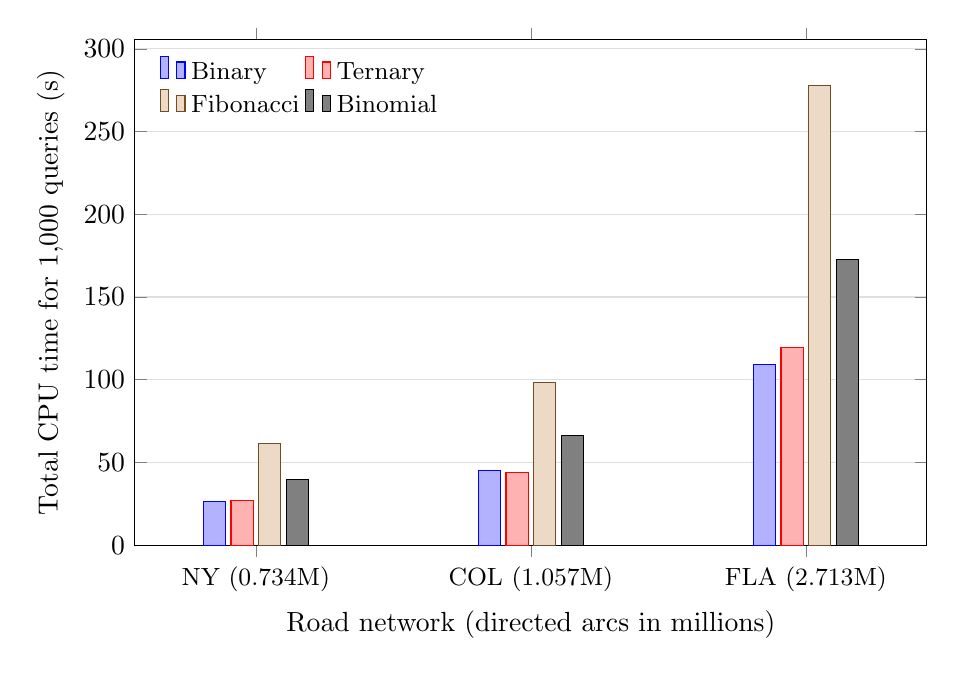
\begin{tikzpicture}
    \begin{axis}[
      ybar,
      bar width=8pt,
      width=0.96\linewidth,
      height=8cm,
      ymin=0,
      ylabel={Total CPU time for 1,000 queries (s)},
      xlabel={Road network (directed arcs in millions)},
      symbolic x coords={NY,COL,FLA},
      xtick=data,
      xticklabels={NY (0.734M),COL (1.057M),FLA (2.713M)},
      x tick label style={font=\small},
      ymajorgrids=true,
      grid style={gray!25},
      enlarge x limits=0.22,
      legend style={at={(0.02,0.98)},anchor=north west,legend columns=2,
                    font=\small,draw=none,fill=white},
      legend cell align=left
    ]
      \addplot coordinates {(NY,26.373) (COL,45.077) (FLA,108.990)};
      \addplot coordinates {(NY,27.077) (COL,43.880) (FLA,119.341)};
      \addplot coordinates {(NY,61.607) (COL,98.328) (FLA,277.698)};
      \addplot coordinates {(NY,39.764) (COL,66.029) (FLA,172.555)};
      \legend{Binary,Ternary,Fibonacci,Binomial}
    \end{axis}
  \end{tikzpicture}
  \caption{Batch runtime as the number of directed input arcs increases}
  \label{fig:runtime}
\end{figure}

The binary heap is fastest on NY and FLA, while the ternary heap is about 2.7\%
faster on COL. The two array heaps are much closer to each other than to the
linked heaps, although their ranking changes across datasets. Fibonacci is
about 2.18--2.55 times as slow as binary; binomial is about 1.47--1.58 times
as slow. The three graphs differ in both size and road
structure, so the increase in runtime across the plot cannot be attributed to
arc count alone. Each heap--dataset pair was timed once, so small differences
should be treated as observations rather than stable rankings.

\section{Dijkstra Work Performed}
The following counts are totals over the 1,000 queries on each dataset. All
four implementations perform the same high-level Dijkstra work on a given
graph.

\begin{table}[H]
  \centering
  \caption{Shared Dijkstra-level operation counts over 1,000 queries}
  \label{tab:work}
  \small
  \begin{tabular}{lrrrr}
    \toprule
    Dataset & Scanned arcs & Extract-min & Insert & Successful decrease-key \\
    \midrule
    NY  & 385,059,749 & 135,502,866 & 135,947,390 & 19,297,309 \\
    COL & 541,176,229 & 220,809,144 & 221,168,701 & 16,421,882 \\
    FLA & 1,347,518,609 & 531,602,948 & 532,034,751 & 50,489,498 \\
    \bottomrule
  \end{tabular}
\end{table}

Extract-min outnumbers successful decrease-key by approximately 7.02, 13.45,
and 10.53 times on NY, COL, and FLA, respectively. Successful decrease-key
accounts for about 6.64\%, 3.58\%, and 4.53\% of the three queue operation
types combined. This workload fact is important when interpreting the
Fibonacci heap's amortized decrease-key advantage.

% ============================== Chapter 4 ================================
\chapter{Analysis and Comments}

\section{Time and Space Complexity Analysis}
For a complete single-source search, the graph representation takes
$O(V+E)$ space and each heap stores at most $V$ vertices. The queue-operation
bounds in Table~\ref{tab:heap-operations} yield the complete-search bounds in
Table~\ref{tab:complexity}. The measured point-to-point queries stop early, so
their actual number of settled vertices and scanned arcs may be substantially
smaller than $V$ and $E$ per query.

With $V_r$ settled vertices and $E_r$ scanned arcs in a particular query, the
binary, ternary, and binomial implementations perform
$O((V_r+E_r)\log V)$ queue work in the standard bound, since the active
frontier can contain vertices that have not yet been settled. The Fibonacci
implementation has amortized $O(E_r+V_r\log V)$ queue work. These are
asymptotic descriptions; the benchmark compares complete query batches and
does not isolate the cost of a single heap operation.

\section{Performance Comparison and Result Analysis}
All four implementations process the same queries and perform identical
Dijkstra-level work on each graph. The observed time gaps therefore arise
primarily from the heap operations and their implementation costs. The
operation counts below come from the independent legacy counter build; they
describe structural work, but are not a time decomposition of the optimized
timing build.

\subsection{Observed Runtime Ratios}
Table~\ref{tab:runtime-ratios} expresses the main timing results relative to
the binary heap. It makes the size and consistency of the gaps easier to see.

\begin{table}[H]
  \centering
  \caption{Runtime relative to the binary heap in the main benchmark}
  \label{tab:runtime-ratios}
  \begin{tabular}{lrrr}
    \toprule
    Dataset & Ternary / Binary & Fibonacci / Binary & Binomial / Binary \\
    \midrule
    NY  & 1.027 ($+2.7\%$) & 2.335 & 1.508 \\
    COL & 0.973 ($-2.7\%$) & 2.181 & 1.465 \\
    FLA & 1.095 ($+9.5\%$) & 2.548 & 1.583 \\
    \bottomrule
  \end{tabular}
\end{table}

The array-heap results are closer to each other than to the linked heaps, and
their order changes by dataset. The Fibonacci implementation is 2.18--2.55
times the binary runtime, and the binomial implementation is 1.46--1.58 times
the binary runtime. Each heap--dataset pair was timed only once; in
particular, repeated runs are needed to assess whether the 9.5\% FLA
binary/ternary gap is stable. The larger linked-heap gaps recur on all three
graphs, though they still describe only these implementations and this
workload.

\subsection{Why the Array Heaps Are Close}
The active queue peaks at only 1,002, 1,037, and 1,575 items on NY, COL, and
FLA. A binary heap at these sizes has roughly 10--11 levels. Both array heaps
therefore have short paths, contiguous storage, and direct vertex lookup via
the position array. A ternary heap shortens the downward path but examines up
to three children per level. This trade-off appears in the internal counters:

\begin{table}[H]
  \centering
  \caption{Ternary-heap internal counts relative to binary (legacy counter build)}
  \label{tab:array-counters}
  \small
  \begin{tabular}{lrrr}
    \toprule
    Dataset & Comparisons & Fewer downward iterations & Fewer array swaps \\
    \midrule
    NY  & $+0.55\%$ & $27.9\%$ & $32.2\%$ \\
    COL & $+0.93\%$ & $27.4\%$ & $32.4\%$ \\
    FLA & $+0.79\%$ & $27.6\%$ & $32.2\%$ \\
    \bottomrule
  \end{tabular}
\end{table}

The ternary heap consistently performs fewer downward iterations and swaps,
but performs slightly more comparisons. With both structures operating on
contiguous arrays and on shallow queues, these costs nearly balance: ternary
is 2.7\% faster on COL, but 2.7\% slower on NY and 9.5\% slower on FLA in
the single-run timing table. Cache locality is a plausible contributor to
the array heaps' advantage over pointer-based heaps, but hardware cache
counters were not collected.

\subsection{Why the Fibonacci Heap Is Slower Here}
The amortized $O(1)$ decrease-key operation is useful only when it forms a
substantial part of the workload. Here, successful decrease-key calls are
only 3.58--6.64\% of the three queue operation types, while extract-min is
performed 135.5--531.6 million times per dataset. Each Fibonacci extract-min
promotes children and consolidates roots, so this frequent operation incurs
linked-structure maintenance. Table~\ref{tab:fib-counters} summarizes the
legacy counters for the Fibonacci implementation.
In the following tables, M and B denote million and billion, respectively.

\begin{table}[H]
  \centering
  \caption{Fibonacci-heap structural work (legacy counter build)}
  \label{tab:fib-counters}
  \small
  \begin{tabular}{lrrrr}
    \toprule
    Dataset & Comparisons / Binary & Children / extract & Cuts / decrease & Tree links (B) \\
    \midrule
    NY  & 1.20$\times$ & 7.50 & 21.0\% & 1.02 \\
    COL & 1.20$\times$ & 7.10 & 23.1\% & 1.57 \\
    FLA & 1.20$\times$ & 7.45 & 19.8\% & 3.97 \\
    \bottomrule
  \end{tabular}
\end{table}

The Fibonacci heap performs about 20\% more counted key/item comparisons than
the binary heap. Table~\ref{tab:fib-counters} shows about 7.1--7.5 child
promotions per extract-min and roughly one billion to four billion tree links
per dataset. Cuts happen on only about one fifth of successful decrease-key calls. Thus, this query
mix does not provide enough decrease-key work to compensate for repeated
extract-min consolidation and linked-list traversal.

The earlier Fibonacci implementation also cleared and scanned a degree table
whose capacity was based on the full graph size on every consolidation. The
estimate in Table~\ref{tab:fib-degree} quantifies this avoidable work; the
optimized version processes only the degrees touched during that
consolidation.

\begin{table}[H]
  \centering
  \caption{Estimated redundant degree-table work in the earlier Fibonacci implementation}
  \label{tab:fib-degree}
  \small
  \begin{tabular}{lrrrr}
    \toprule
    Dataset & Table slots & Extract-min calls & Full-scan iterations & Logical bytes cleared \\
    \midrule
    NY  & 39 & 135.5 M & 5.28 B & 42.3 GB \\
    COL & 39 & 220.8 M & 8.61 B & 68.9 GB \\
    FLA & 43 & 531.6 M & 22.86 B & 182.9 GB \\
    \bottomrule
  \end{tabular}
\end{table}

The byte totals are repeated logical bytes passed to clearing operations, not
DRAM traffic; the small table may remain in cache. They estimate the earlier
implementation and must not be read as work performed by the optimized
version.

\subsection{Why the Binomial Heap Is Slower Despite Fewer Comparisons}
The binomial heap records only about 70\% as many counted comparisons as the
binary heap, yet takes 1.46--1.58 times as long. This illustrates why a
comparison counter is not a complete cost model. Binomial operations also
merge degree-ordered root lists, link equal-degree trees, promote children,
and update parent/sibling pointers.

\begin{table}[H]
  \centering
  \caption{Binomial-heap structural work (legacy counter build)}
  \label{tab:binomial-counters}
  \small
  \begin{tabular}{lrrr}
    \toprule
    Dataset & Comparisons / Binary & Tree links (B) & Root-list steps (B) \\
    \midrule
    NY  & 0.70$\times$ & 1.04 & 4.09 \\
    COL & 0.70$\times$ & 1.61 & 6.37 \\
    FLA & 0.70$\times$ & 4.06 & 15.98 \\
    \bottomrule
  \end{tabular}
\end{table}

Its root-list step counter reaches 4.09 billion on NY and 15.98 billion on
FLA, consistent with substantial list traversal. The counter definitions
differ between Fibonacci and binomial heaps, so their root-list totals are
not directly comparable.

\subsection{Separate One-Round Optimization Comparison}
The performance analysis notes also record an original-versus-optimized
comparison on the same machine. It is a separate run set from the primary
runtime table and is included only to show the observed relative change.
Each version was timed once.
Each total sums NY, COL, and FLA, or 3,000 queries per heap and version.

\begin{table}[H]
  \centering
  \caption{Separate one-round original-versus-optimized comparison}
  \label{tab:optimization}
  \begin{tabular}{lrrr}
    \toprule
    Heap & Original total (s) & Optimized total (s) & Observed change \\
    \midrule
    Binary    & 81.527  & 70.591  & $-13.4\%$ \\
    Ternary   & 84.023  & 73.247  & $-12.8\%$ \\
    Fibonacci & 255.043 & 194.704 & $-23.7\%$ \\
    Binomial  & 172.224 & 153.616 & $-10.8\%$ \\
    \bottomrule
  \end{tabular}
\end{table}

Common changes included compiling out internal counters from the timing build
and using direct heap calls on the Dijkstra hot path. The Fibonacci change
also reduced degree-table scanning, while the binomial change removed an
extra traversal used only for counting. The table cannot separate the
contribution of each change, and its one-round percentages are not repeated-run
statistics.

\section{Further Improvements and Measurement Limits}
The current measurements support a comparison of these implementations on
these road-network point-to-point queries. They do not establish a universal
ranking. The main limitations are:

\begin{enumerate}
  \item Each heap--dataset pair in the primary table was timed once. Repeated
        runs after warm-up, summarized with medians and dispersion, would make
        small differences more reliable.
  \item The primary runtimes and the separate original-versus-optimized
        timings are different experiment sets and must not be combined into a
        single speedup calculation.
  \item Internal heap counters describe the earlier implementation. They
        explain operation patterns but are not a precise cost breakdown for
        the optimized build.
  \item Matching answers across four implementations is a cross-check, not an
        independent correctness proof. Additional small-graph reference tests
        should be run against the optimized version.
  \item The experiment does not collect hardware cache-miss, branch, or
        pointer-access measurements. Memory locality is a plausible
        explanation for some differences, not a separately measured cause.
  \item The local DIMACS files were count-checked after reconstruction but
        were not verified arc by arc against the official files.
\end{enumerate}

Useful next measurements would include multiple timed repetitions, full
single-source queries, more road networks, and hardware profiling. They may
change the operation mix or clarify which low-level costs explain the
observed differences.

\section{Summary}
On the three tested road networks, binary and ternary heaps were faster than
the current Fibonacci and binomial implementations for the measured
point-to-point workload. Successful decrease-key was a small share of queue
operations, while extract-min occurred hundreds of millions of times across
the query batches. This operation mix helps explain why Fibonacci's amortized
decrease-key advantage did not dominate the total runtime. The binary and
ternary results were close, and the single-run measurements do not establish
a stable winner between them. These conclusions apply to the recorded
implementations and query workload; different graph structures or query
patterns may lead to different results.

\chapter*{References}
\addcontentsline{toc}{chapter}{References}
\begin{enumerate}[label={[\arabic*]}]
  \item Ye De-shi. \textit{Shortest Path Algorithm with Heaps}, Assignment
        8-1, Zhejiang University, course handout.
  \item DIMACS. \textit{9th DIMACS Implementation Challenge: Shortest Paths}.
        \href{https://www.diag.uniroma1.it/challenge9/download.shtml}{DIMACS download page}.
\end{enumerate}

\appendix
\chapter{Source Location}
The complete implementation is in \code{src/1.c}.
It contains DIMACS graph loading, all four priority queues, Dijkstra query
execution, deterministic query generation, runtime measurement, and CSV
output. Implementation details are summarized in Chapter 2; this report
focuses on their measured performance consequences.

Recorded files include:
\begin{itemize}
  \item Timings: \path{results/benchmark_results.csv}.
  \item Queries: \path{results/benchmark_queries.csv}.
  \item Dijkstra operation counts: \path{results/benchmark_operations.csv}.
  \item Legacy heap counters: \path{results/heap_internal_stats.csv}.
  \item Performance analysis: \path{docs/heap_performance_analysis.md}.
\end{itemize}

\end{document}
